% Sources :
%    * http://texample.net/tikz/examples/sudoku/
%    * http://tex.stackexchange.com/questions/91421/tikz-changing-the-z-index-of-backgrounds
%    * http://tex.stackexchange.com/questions/86542/tikz-placing-several-numbers-in-one-cell-of-a-sudoku-grid
%    * http://tex.stackexchange.com/questions/91422/tikz-sudoku-circle-and-line/91429#91429

\documentclass{article}
    \usepackage{tikz}
    \usetikzlibrary{backgrounds,shapes}
    \usepackage{graphicx}
    \usepackage{xstring}

% Some customizable styles
    \tikzset {
        highlight/.style = {
            yellow,
            opacity = 0.3
        },
        digit/.style = {
            minimum height = 5mm,
            minimum width = 5mm,
            anchor = center
        },
        circle/.style = {
            draw = green!80!black,
            dotted,
            very thick
        },
        circle number/.style = {
            draw = #1,
            very thick
        },
        cross/.style = {
            red,
            opacity = .5,
            shorten >= 1mm,
            shorten <= 1mm,
            very thick,
            line cap = round
        },
        hint/.style = {
            blue,
            font = \sf,
            minimum width = 3mm,
            minimum height = 3mm
        },
        hint special/.style = {
            blue,
            font = \sf,
            minimum width = 3mm,
            minimum height = 3mm,
            fill=red!20,
            inner sep=0pt,
        },
        hint border/.style = {
            blue,
            font = \sf,
            minimum width = 2mm,
            minimum height = 3mm,
            inner sep=0pt, outer sep=0pt,
            draw=red, thick,
            rounded corners=1pt,
        }
    }

% Modified the \node to give a unique name to each one, which is the
% row number, a dash and the column number. E.g: 1-1, 4-5, etc.
    \newcounter{row}
    \newcounter{col}

    \newcommand\setrow[9]{
        \setcounter{col}{1}
        \foreach \n in {#1, #2, #3, #4, #5, #6, #7, #8, #9} {
            \edef\x{\value{col} - 0.5}
            \edef\y{9.5 - \value{row}}
            \node[digit,name={\arabic{row}-\arabic{col}}] at (\x, \y) {\n};
            \stepcounter{col}
        }
        \stepcounter{row}
    }

% New code -------------------------------------------------------------
    \def\highlightcell#1#2{
        \begin{scope}[on background layer]
            \fill[highlight] (#1-#2.north west) rectangle (#1-#2.south east);
        \end{scope}
    }

    \def\circlecell#1#2{
        \draw[circle] (#1-#2) circle(4mm);
    }

    \def\crosscell#1#2{
        \draw[cross] (#1-#2.north west) -- (#1-#2.south east);
        \draw[cross] (#1-#2.north east) -- (#1-#2.south west);
    }

    \def\highlightrow#1{
        \begin{scope}[on background layer]
            \fill[highlight] (#1-1.north west) rectangle (#1-9.south east);
        \end{scope}
    }

    \def\highlighcolumn#1{
        \begin{scope}[on background layer]
            \fill[highlight] (1-#1.north west) rectangle (9-#1.south east);
        \end{scope}
    }

    \def\highlightrectangle#1#2#3#4{
        \begin{scope}[on background layer]
            \fill[highlight] (#1-#2.north west) rectangle (#3-#4.south east);
        \end{scope}
    }

    \def\hintcell#1#2#3{
        \node at (#1-#2) {\hintbox{#3}};
    }


% Command to circle numbers:
% #1: optional -> circle color
% #2: mandatory -> cell identifier
% #3: mandatory -> name of the cell
    \newcommand\circlenumber[3][red!80!black]{
        \draw[circle number=#1, radius=5mm] (#2) circle node[outer sep=1mm] (#3){};
    }

% UGLY code. Do not read :-)
%  Sorry, it needed to be read to obtain solution :-)
    \def\hintbox#1{
        \resizebox{4.5mm}{4.5mm}{%
            \tikz[scale=0.3]{%
                \def\auxc{0}
                \foreach \m in {1,...,9} {
                    \pgfmathparse{mod(\auxc,3)}
                    \xdef\x{\pgfmathresult}
                    \pgfmathparse{-floor(\auxc/3)}
                    \xdef\y{\pgfmathresult}
                    \xdef\hintprinted{0}
                    \foreach \n/\Style in {#1} {
                        \ifnum\n=\m
                            \IfStrEqCase{\Style}{%
                                {}{\node[hint] at (\x,\y) {\n};}                                
                                {\n}{\node[hint] at (\x,\y) {\n};}
                                {border}{\node[hint border] at (\x,\y) {\n};}                           
                                {special}{\node[hint special] at (\x,\y) {\n};}
                            }
                            \xdef\hintprinted{1}
                        \fi
                    }
                    \ifnum\hintprinted=0
                        \node[hint, opacity=0.1] at (\x,\y) {\m};
                    \fi
                    \pgfmathparse{\auxc+1}
                    \xdef\auxc{\pgfmathresult}
                }
            }%
        }
    }

% To see the numbers of lines and columns.
    \newcommand\shownumber{
        \foreach \x in {1,2,3,4,5,6,7,8,9} {
            \node[font=\tiny,color=gray] at (\x-0.5,9.5) {\x};
            \node[font=\tiny,color=gray] at (-.5,9.5-\x) {\x};
        }
    }


\begin{document}

\scalebox{3}{
    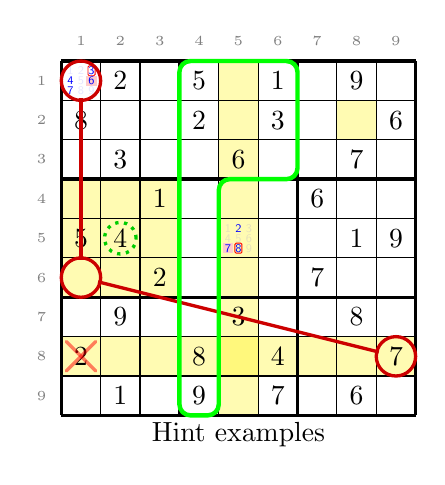
\begin{tikzpicture}[scale=.5]
        \begin{scope}
            \draw (0, 0) grid (9, 9);
            \draw[very thick, scale=3] (0, 0) grid (3, 3);

            \setcounter{row}{1}
            \setrow { }{2}{ }  {5}{ }{1}  { }{9}{ }
            \setrow {8}{ }{ }  {2}{ }{3}  { }{ }{6}
            \setrow { }{3}{ }  { }{6}{ }  { }{7}{ }
    
            \setrow { }{ }{1}  { }{ }{ }  {6}{ }{ }
            \setrow {5}{4}{ }  { }{ }{ }  { }{1}{9}
            \setrow { }{ }{2}  { }{ }{ }  {7}{ }{ }

            \setrow { }{9}{ }  { }{3}{ }  { }{8}{ }
            \setrow {2}{ }{ }  {8}{ }{4}  { }{ }{7}
            \setrow { }{1}{ }  {9}{ }{7}  { }{6}{ }

            \node[anchor=center] at (4.5, -0.5) {Hint examples};

            \highlightcell{2}{8};
            \highlightrow{8}
            \highlighcolumn{5}
            \highlightrectangle{4}{1}{6}{3}

            \hintcell{5}{5}{2,7/special,8/border}
            \hintcell{1}{1}{3/border,4,6/special,7}

            \circlecell{5}{2}
            \crosscell{8}{1}

            \circlenumber{1-1}{start}
            \circlenumber{6-1}{middle}
            \circlenumber{8-9}{end}

            \foreach \source/\dest in {start/middle,middle/end}
                \draw[circle number=red!80!black] (\source)--(\dest);
        
            \draw[ultra thick, green, rounded corners]
            (3,9)
                   -- ++(right:3) -- ++(down:3)
                   -- ++(left:2)  -- ++(down:6)
                   -- ++(left:1) 
                   -- cycle;

            \shownumber{}
        \end{scope}
    \end{tikzpicture}
}


\newpage


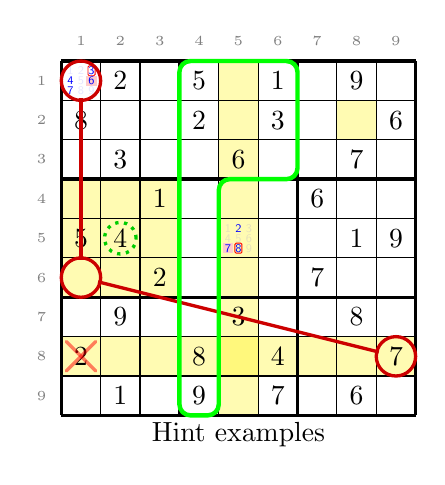
\begin{tikzpicture}[scale=.5]
    \begin{scope}
        \draw (0, 0) grid (9, 9);
        \draw[very thick, scale=3] (0, 0) grid (3, 3);

        \setcounter{row}{1}
        \setrow { }{2}{ }  {5}{ }{1}  { }{9}{ }
        \setrow {8}{ }{ }  {2}{ }{3}  { }{ }{6}
        \setrow { }{3}{ }  { }{6}{ }  { }{7}{ }

        \setrow { }{ }{1}  { }{ }{ }  {6}{ }{ }
        \setrow {5}{4}{ }  { }{ }{ }  { }{1}{9}
        \setrow { }{ }{2}  { }{ }{ }  {7}{ }{ }

        \setrow { }{9}{ }  { }{3}{ }  { }{8}{ }
        \setrow {2}{ }{ }  {8}{ }{4}  { }{ }{7}
        \setrow { }{1}{ }  {9}{ }{7}  { }{6}{ }

        \node[anchor=center] at (4.5, -0.5) {Hint examples};

        \highlightcell{2}{8};
        \highlightrow{8}
        \highlighcolumn{5}
        \highlightrectangle{4}{1}{6}{3}

        \hintcell{5}{5}{2,7/special,8/border}
        \hintcell{1}{1}{3/border,4,6/special,7}

        \circlecell{5}{2}
        \crosscell{8}{1}

        \circlenumber{1-1}{start}
        \circlenumber{6-1}{middle}
        \circlenumber{8-9}{end}

        \foreach \source/\dest in {start/middle,middle/end}
            \draw[circle number=red!80!black] (\source)--(\dest);
        
        \draw[ultra thick, green, rounded corners]
            (3,9)
               -- ++(right:3) -- ++(down:3)
               -- ++(left:2)  -- ++(down:6)
               -- ++(left:1) 
               -- cycle;

        \shownumber{}
    \end{scope}
\end{tikzpicture}


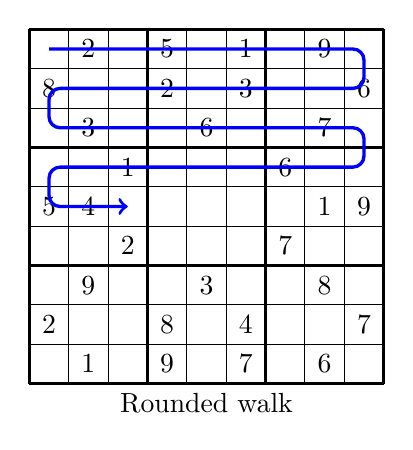
\begin{tikzpicture}[scale=.5]
    \begin{scope}
        \draw (0, 0) grid (9, 9);
        \draw[very thick, scale=3] (0, 0) grid (3, 3);

        \setcounter{row}{1}
        \setrow { }{2}{ }  {5}{ }{1}  { }{9}{ }
        \setrow {8}{ }{ }  {2}{ }{3}  { }{ }{6}
        \setrow { }{3}{ }  { }{6}{ }  { }{7}{ }

        \setrow { }{ }{1}  { }{ }{ }  {6}{ }{ }
        \setrow {5}{4}{ }  { }{ }{ }  { }{1}{9}
        \setrow { }{ }{2}  { }{ }{ }  {7}{ }{ }

        \setrow { }{9}{ }  { }{3}{ }  { }{8}{ }
        \setrow {2}{ }{ }  {8}{ }{4}  { }{ }{7}
        \setrow { }{1}{ }  {9}{ }{7}  { }{6}{ }

        \node[anchor=center] at (4.5, -0.5) {Rounded walk};

        \draw[->,very thick, blue, rounded corners] 
            (1-1.center) -- (1-9.center) 
                        |-  (2-1.center) 
                        |-  (3-9.center) 
                        |-  (4-1.center) 
                        |-  (5-3.center);
    \end{scope}
\end{tikzpicture}


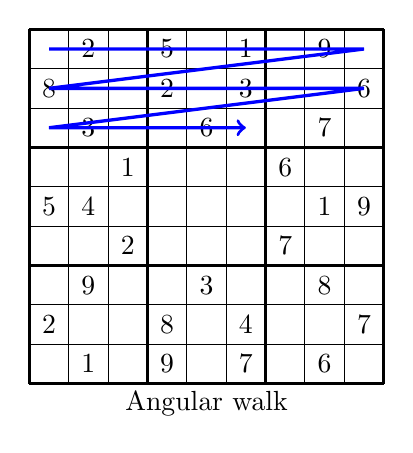
\begin{tikzpicture}[scale=.5]
    \begin{scope}
        \draw (0, 0) grid (9, 9);
        \draw[very thick, scale=3] (0, 0) grid (3, 3);

        \setcounter{row}{1}
        \setrow { }{2}{ }  {5}{ }{1}  { }{9}{ }
        \setrow {8}{ }{ }  {2}{ }{3}  { }{ }{6}
        \setrow { }{3}{ }  { }{6}{ }  { }{7}{ }

        \setrow { }{ }{1}  { }{ }{ }  {6}{ }{ }
        \setrow {5}{4}{ }  { }{ }{ }  { }{1}{9}
        \setrow { }{ }{2}  { }{ }{ }  {7}{ }{ }

        \setrow { }{9}{ }  { }{3}{ }  { }{8}{ }
        \setrow {2}{ }{ }  {8}{ }{4}  { }{ }{7}
        \setrow { }{1}{ }  {9}{ }{7}  { }{6}{ }

        \node[anchor=center] at (4.5, -0.5) {Angular walk};

        \draw[->,very thick, blue] 
            (1-1.center) -- (1-9.center) 
         -- (2-1.center) -- (2-9.center) 
         -- (3-1.center) -- (3-6.center);
    \end{scope}
\end{tikzpicture}


\newpage


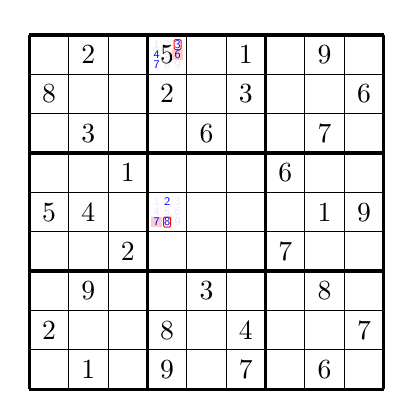
\begin{tikzpicture}[scale=.5]
    \begin{scope}
        \draw (0, 0) grid (9, 9);
        \draw[very thick, scale=3] (0, 0) grid (3, 3);

        \setcounter{row}{1}
        \setrow { }{2}{ }  {5}{ }{1}  { }{9}{ }
        \setrow {8}{ }{ }  {2}{ }{3}  { }{ }{6}
        \setrow { }{3}{ }  { }{6}{ }  { }{7}{ }

        \setrow { }{ }{1}  { }{ }{ }  {6}{ }{ }
        \setrow {5}{4}{ }  { }{ }{ }  { }{1}{9}
        \setrow { }{ }{2}  { }{ }{ }  {7}{ }{ }

        \setrow { }{9}{ }  { }{3}{ }  { }{8}{ }
        \setrow {2}{ }{ }  {8}{ }{4}  { }{ }{7}
        \setrow { }{1}{ }  {9}{ }{7}  { }{6}{ }

        \hintcell{5}{4}{2,7/special,8/border}
        \hintcell{1}{4}{3/border,4,6/special,7}
    \end{scope}
\end{tikzpicture}

\medskip

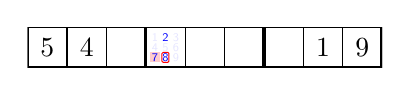
\begin{tikzpicture}[scale=.5]
    \begin{scope}
        \clip (0,3.99) rectangle (9,5);
        \draw (0, 0) grid (9, 9);
        \draw[very thick, scale=3] (0, 0) grid (3, 3);

        \setcounter{row}{1}
        \setrow { }{2}{ }  {5}{ }{1}  { }{9}{ }
        \setrow {8}{ }{ }  {2}{ }{3}  { }{ }{6}
        \setrow { }{3}{ }  { }{6}{ }  { }{7}{ }

        \setrow { }{ }{1}  { }{ }{ }  {6}{ }{ }
        \setrow {5}{4}{ }  { }{ }{ }  { }{1}{9}
        \setrow { }{ }{2}  { }{ }{ }  {7}{ }{ }

        \setrow { }{9}{ }  { }{3}{ }  { }{8}{ }
        \setrow {2}{ }{ }  {8}{ }{4}  { }{ }{7}
        \setrow { }{1}{ }  {9}{ }{7}  { }{6}{ }

        \hintcell{5}{4}{2,7/special,8/border}
        \hintcell{1}{4}{3/border,4,6/special,7}
    \end{scope}
\end{tikzpicture}

\medskip

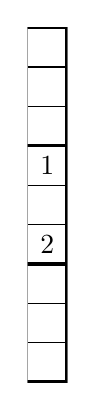
\begin{tikzpicture}[scale=.5]
    \begin{scope}
        \clip (2,0) rectangle (3.01,9);
        \draw (0, 0) grid (9, 9);
        \draw[very thick, scale=3] (0, 0) grid (3, 3);

        \setcounter{row}{1}
        \setrow { }{2}{ }  {5}{ }{1}  { }{9}{ }
        \setrow {8}{ }{ }  {2}{ }{3}  { }{ }{6}
        \setrow { }{3}{ }  { }{6}{ }  { }{7}{ }

        \setrow { }{ }{1}  { }{ }{ }  {6}{ }{ }
        \setrow {5}{4}{ }  { }{ }{ }  { }{1}{9}
        \setrow { }{ }{2}  { }{ }{ }  {7}{ }{ }

        \setrow { }{9}{ }  { }{3}{ }  { }{8}{ }
        \setrow {2}{ }{ }  {8}{ }{4}  { }{ }{7}
        \setrow { }{1}{ }  {9}{ }{7}  { }{6}{ }

        \hintcell{5}{4}{2,7/special,8/border}
        \hintcell{3}{4}{3/border,4,6/special,7}
    \end{scope}
\end{tikzpicture}

\medskip

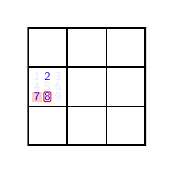
\begin{tikzpicture}[scale=.5]
    \begin{scope}
        \clip (3,3) rectangle (6.01,6);
        \draw (0, 0) grid (9, 9);
        \draw[very thick, scale=3] (0, 0) grid (3, 3);

        \setcounter{row}{1}
        \setrow { }{2}{ }  {5}{ }{1}  { }{9}{ }
        \setrow {8}{ }{ }  {2}{ }{3}  { }{ }{6}
        \setrow { }{3}{ }  { }{6}{ }  { }{7}{ }

        \setrow { }{ }{1}  { }{ }{ }  {6}{ }{ }
        \setrow {5}{4}{ }  { }{ }{ }  { }{1}{9}
        \setrow { }{ }{2}  { }{ }{ }  {7}{ }{ }

        \setrow { }{9}{ }  { }{3}{ }  { }{8}{ }
        \setrow {2}{ }{ }  {8}{ }{4}  { }{ }{7}
        \setrow { }{1}{ }  {9}{ }{7}  { }{6}{ }

        \hintcell{5}{4}{2,7/special,8/border}
        \hintcell{3}{4}{3/border,4,6/special,7}
    \end{scope}
\end{tikzpicture}

\end{document}
